\section * {\LARGE 4. USE CASES}
\begin{center}
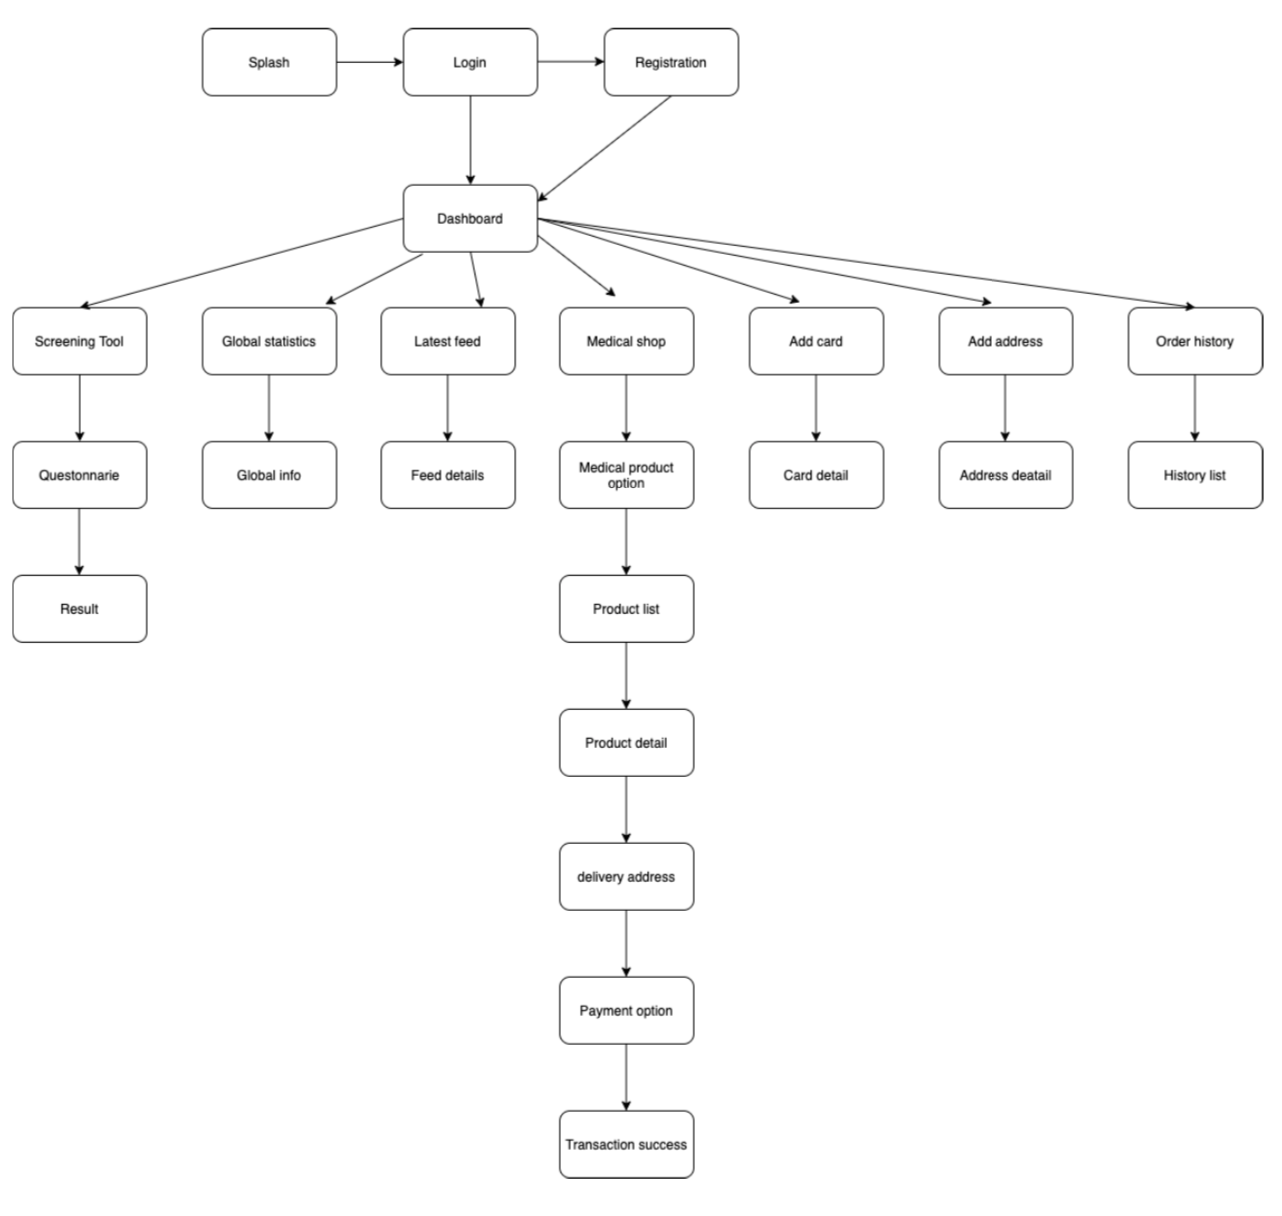
\includegraphics[scale=0.75]{use case.png}\\[0.75cm]
\end{center}
\begin{itemize}
    \item Technical Information About the App:

\begin{enumerate}
    \item MocPlatform: We are developing our application in Android Platform. We have chosen this platform as the maximum number of users are Android mobile users and this will target a greater audience. Another reason is that to deploy the application on Appstore is easy and cheap as well the membership charges are cheap as well the membership charges are 25 dollars for lifetime.

    Reasons of using Native Application 
    \begin{itemize}
    \item Very fast
    \item Built to run on specific platform 
    \item Distributed in Play stores. 
    \item Interactive and intuitive
    \item Interact with device utilities.
\end{itemize}
\item Language: We are developing the application in JAVA programming language.
\item Database: The database we are using is fire base. We are using fire base authentication for login and sign up. For the authentication we used fire- base and for the local storage we used local room.
\end{enumerate}
\end{itemize}


\section*{User Interface}
\begin{itemize}
    \item When the user opens the application the first screen will be login/signup screen.
\item Already registered then the user login otherwise to register the user sign up.
\item After login user can see the screening tool screen where user pick the different option to check the result
\item global stats user can see the 3d globe and can see the situation of world like total infected and total death in real-time
\item There will be a option in navigation drawer to see the latest feed about health sector
\item There will be a option of medical shop in navigation drawer to buy medi-cines.
\item There will be a option of tip and tricks for stay safe at home in navigation drawer
\end{itemize}
